\chapter{Client Side}

\section{AngularJS}
% Talk about my specific implementation. Especially the structure.
% TODO: a good figure is needed to describe my specific implementation. None exists currently.

% TODO: describe this diagram better
\section{High Level View}
\begin{figure}[!ht]
  \centering
  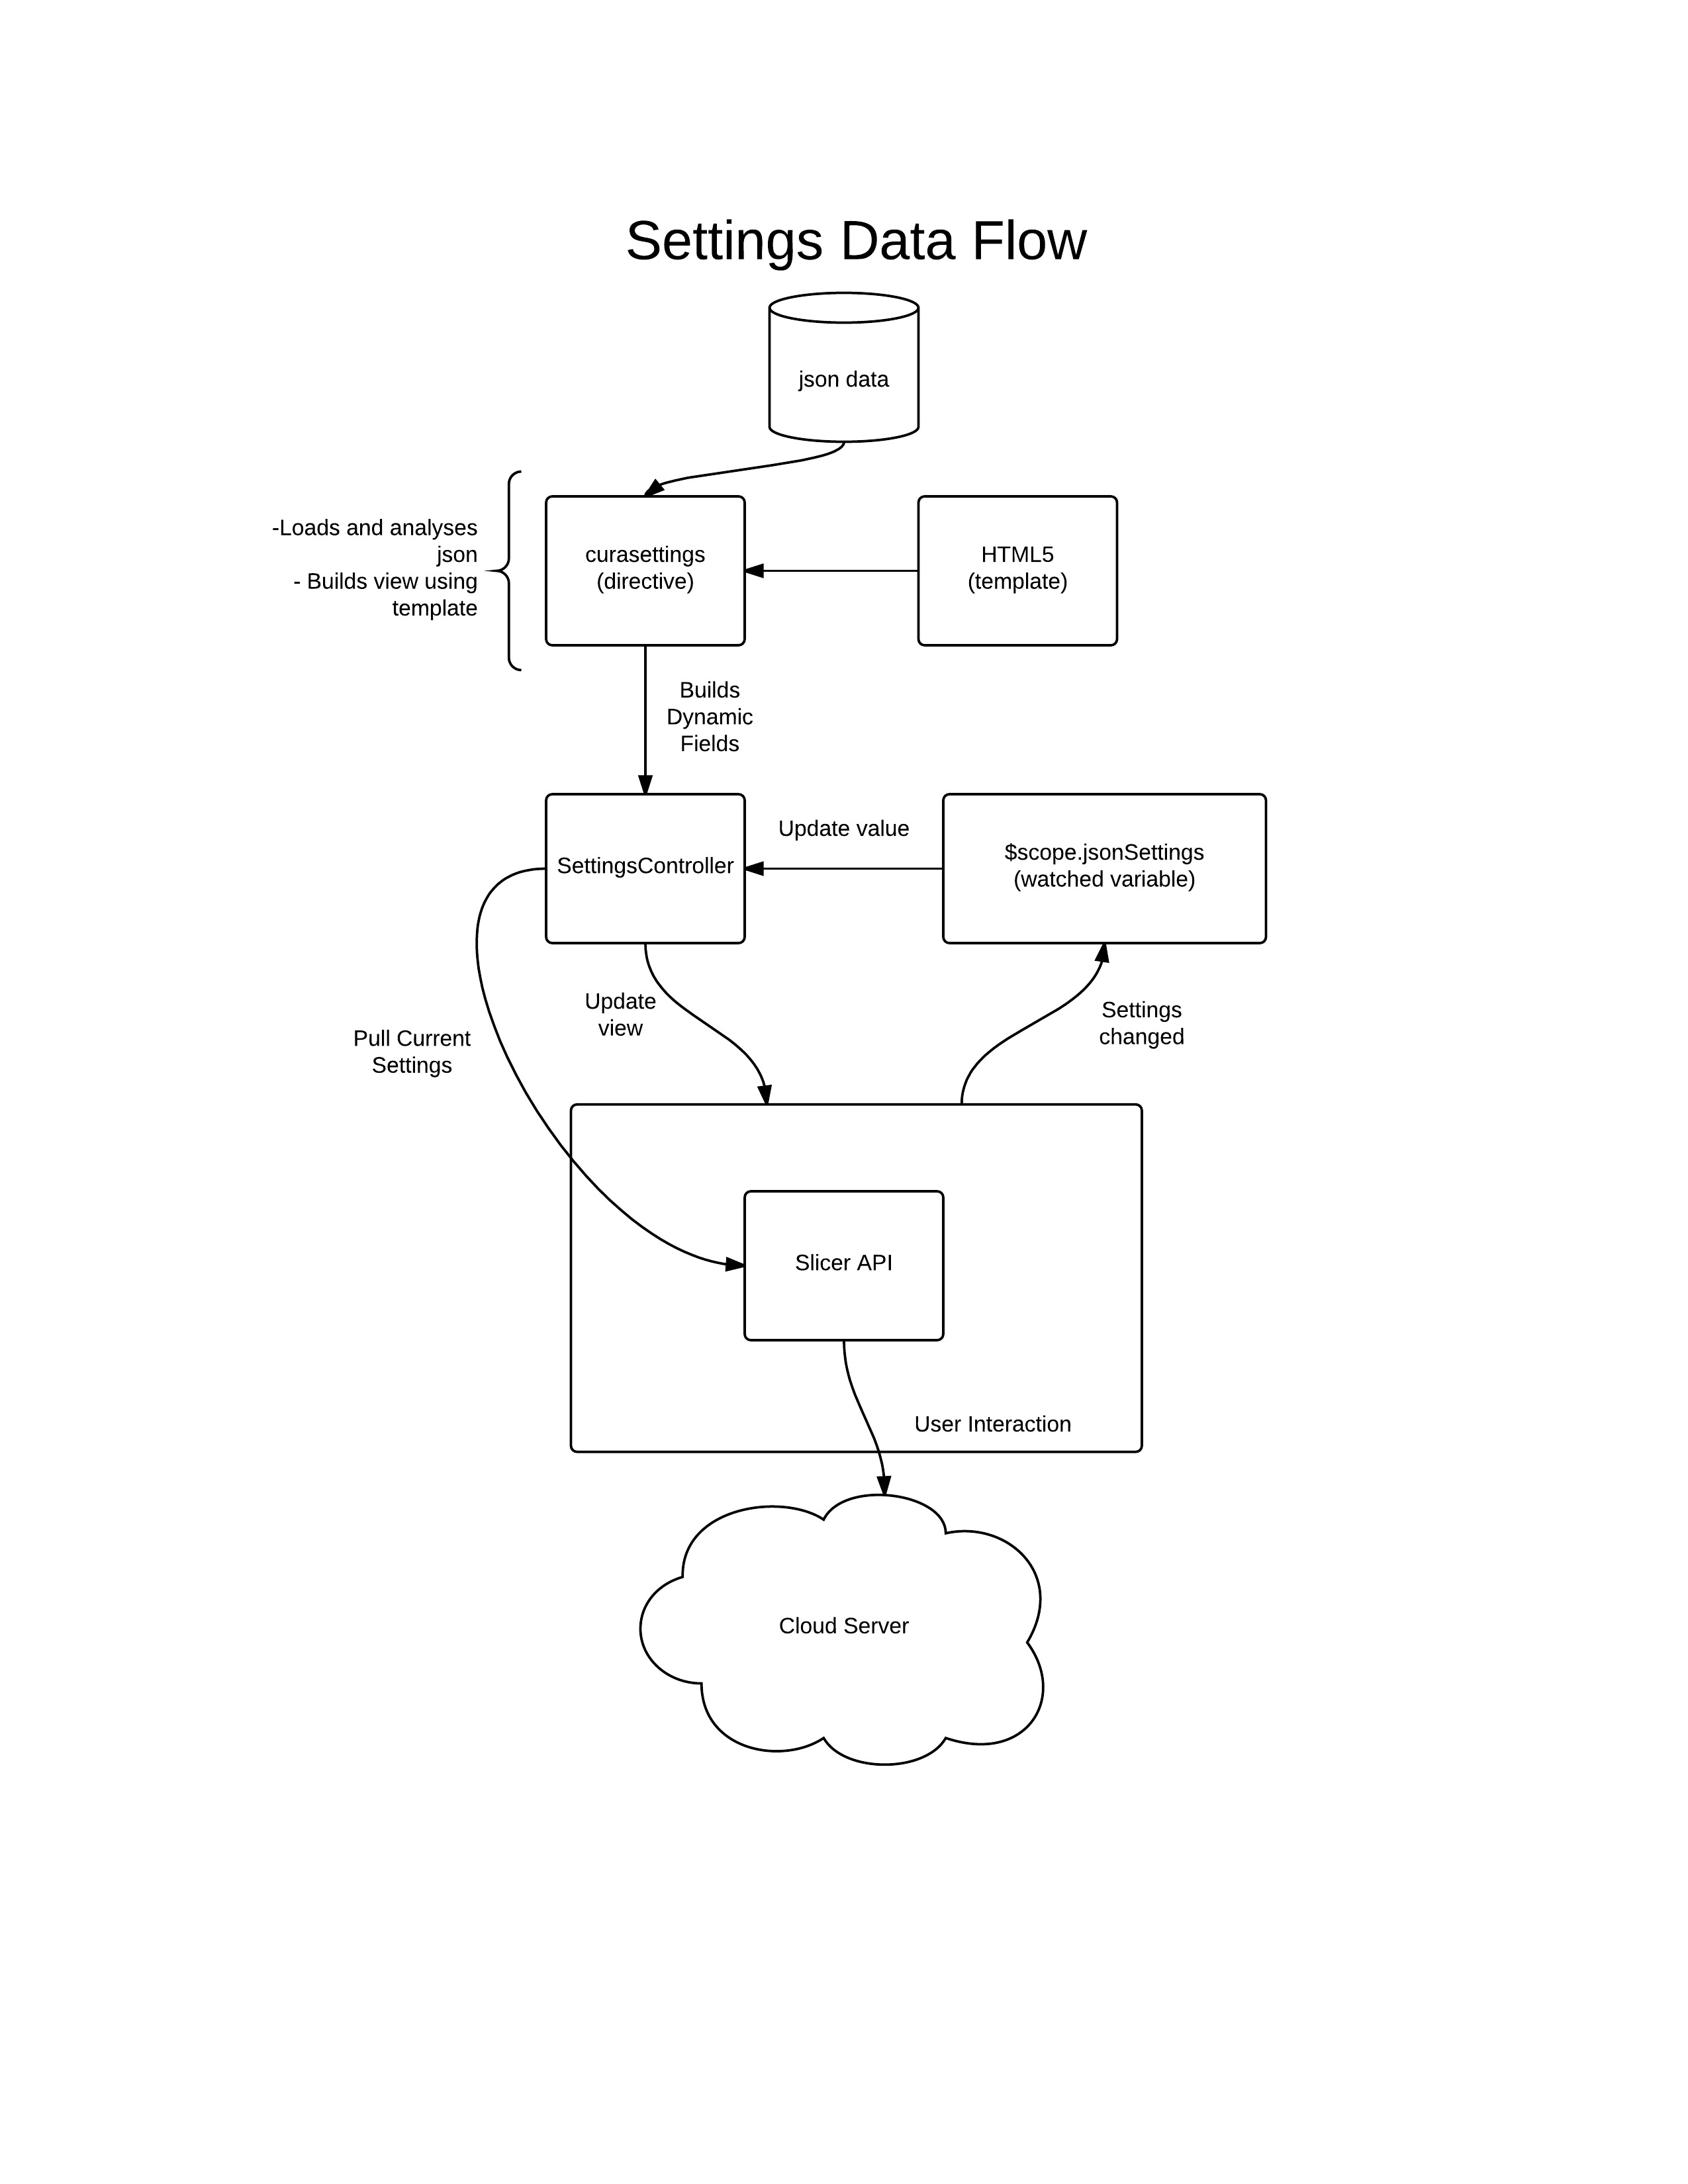
\includegraphics[width=\linewidth]{Settings-Data-Flow}
  \caption{The flow of data through the application from beginning to end of client side user interaction}
  \label{fig:settings-data-flow}
\end{figure}

% TODO: describe settings code and how it works in far more detail
\paragraph{}
As shown in Figure \ref{fig:settings-data-flow}, the client side of this applicaiton has a lengthy flow of data.
This data flow starts with loading a static JSON (JavaScript Object Notation) file which describes the settings in a pattern as shown in Listing \ref{lst:json-settings}.
\begin{lstlisting}[language=json, label={lst:json-settings}, caption=A sample from a static settings file in JSON format.]
{
    "setting": "layer_height",
    "default": 0.1,
    "type": "float",
    "category": "Quality",
    "label": "Layer Height (mm)",
    "description": "Layer height in millimeters. This is the most important setting to determine the quality of your print. Normal quality prints are 0.1mm, high quality is 0.06mm. You can go up to 0.25mm."
}
\end{lstlisting}

\section{OctoPrint Integration}
\section{2D Model Viewer Integration}
\section{Other Planned Integrations}
% Be somewhat brief here

\section{Issues \& Known Bugs}


